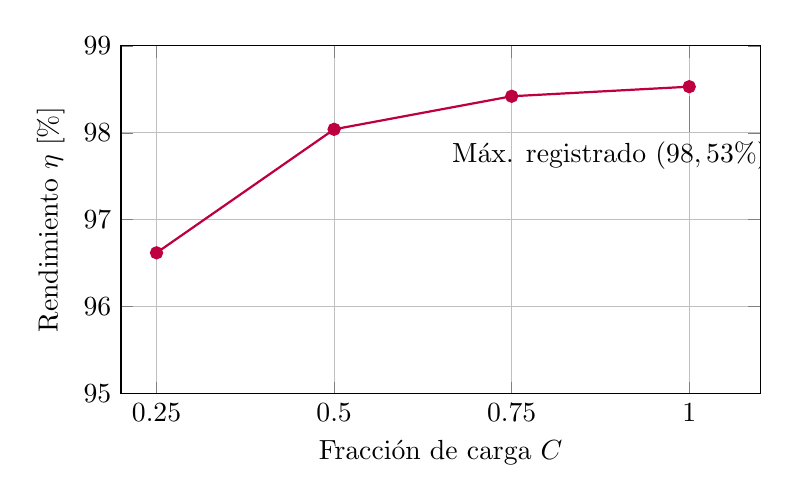
\begin{tikzpicture}
  \begin{axis}[
      xlabel={Fracción de carga $C$},
      ylabel={Rendimiento $\eta$ [\%]},
      xmin=0.2, xmax=1.1,
      ymin=95, ymax=99,
      xtick={0.25, 0.5, 0.75, 1},
      ytick={95, 96, 97, 98, 99},
      grid=major,
      width=0.8\textwidth,
      height=6cm
    ]
    \addplot[color=purple, mark=*, thick] coordinates {
      (0.25, 96.62)
      (0.50, 98.04)
      (0.75, 98.42)
      (1.00, 98.53)
    };
    
    \node[pin=270:{Máx. registrado ($98,53\%$) en $C=1,00$}] at (axis cs:1.00, 98.53) {};
  \end{axis}
\end{tikzpicture}
